% !TeX spellcheck = de_DE
%\documentclass[11pt,a4paper]{article}
\documentclass[11pt
  , a4paper
  , article
  , oneside
%  , twoside
%  , draft
]{memoir}
\setcounter{secnumdepth}{2}
\usepackage{control}
\usepackage[numbers]{natbib}

\newcommand{\newappendix}{%
	\refstepcounter{chapter}\chapter*{Appendix \thechapter}%
	\addcontentsline{toc}{chapter}{Appendix \thechapter}%
}

\newcommand\tab[1][1cm]{\hspace*{#1}}

\begin{document}

\newcommand{\technumber}{
  RAON Control-Document Series\\
  Revision : v1.0,   Release : 2016-12-02 fixed date}
\title{\textbf{EPICS V4 PVAccess Gateway 프로토타입 개발 결과보고서}}

\author{이상일\thanks{silee7103@ibs.re.kr} \\

  Rare Isotope Science Project\\
  Institute for Basic Science, Daejeon, South Korea
}
\date{\today}

\renewcommand{\maketitlehooka}{\begin{flushright}\textsf{\technumber}\end{flushright}}
%\renewcommand{\maketitlehookb}{\centering\textsf{\subtitle}}
%\renewcommand{\maketitlehookc}{C}
%\renewcommand{\maketitlehookd}{D}

\maketitle

\begin{abstract}
본 문서는 EPICS Version 4 통신 프로토콜 "pvAccess"를 정의하고, 그에 따른 "pvAccess Gateway"의 프로토타입 개발 구현에 대한 결과를 설명하는 보고서이다. 또한 본 문서의 pvAccess Gateway 프로토타입 개발은 RAON 중이온가속기에서의 초기 개발 비용을 시작으로 다른 해외연구기관이 그를 이어 받아 향 후 안정화 운영시기까지 계속 개발 및 버전 업데이트가 이루어 질 목적이다. 
\end{abstract}

EPICS를 한마디로 정의하면, 대형실험 과학 장치의 제어시스템을 구축하기 위한 모든 컴퓨터의 플랫폼으로 정의된다.EPICS에 대한 자세한 내용은 "Experimental Physics and Industrial Control System(http://www.aps.anl.gov/epics/)"의 홈 페이지를 참조한다. pvAccess는 계측센서 신호에 대한 모니터링 및 과학적 데이터 서비스를 상호 연결하는 고 성능 네트워크 통신 프로토콜을 말한다. 이는 제어시스템의 양끝단의 최적화된 내부통신을 위해서 pvData라는 EPICS 버전 4 공유메모리 기반의 통신 오브젝트 객체로써, 구조화된 사용자 정의 데이터 타입을 지원하며, EPICS version 3 "channel access" 프로토콜을 계승한다. EPICS V4 pvAccess 프로토콜 및 기본 구현은 EPICS 워킹그룹에 의해 작성된다.  본 문서에서는 게이트웨이의 클라이언트를 "외부"로 지칭하며, 게이트웨이 외부 클라이언트를  연결하는 서버 (예:IOC)를 "내부"로 지칭한다. 이는 게이트웨이의 양면 사이를 명확히 구별하기 위함이다.

\clearpage

\chapter{EPICS v3 Channel Access Gateway 이해}
\section{특성}

\section{이슈 사항}

\begin{figure}[!htb]
	\centering
	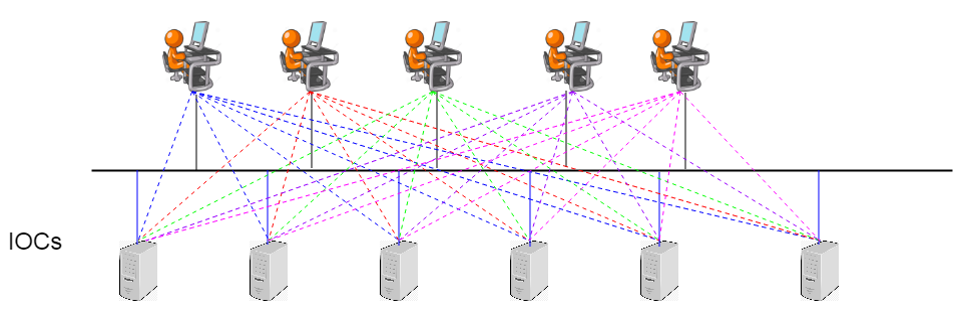
\includegraphics[width=1\textwidth]{./images/flat_network.png}
	\caption{
		Flat Network 상에서의 문제점
	}
	\label{fig:flat_network}   
\end{figure}

\section{Gateway 구성}
\begin{figure}[!htb]
	\centering
	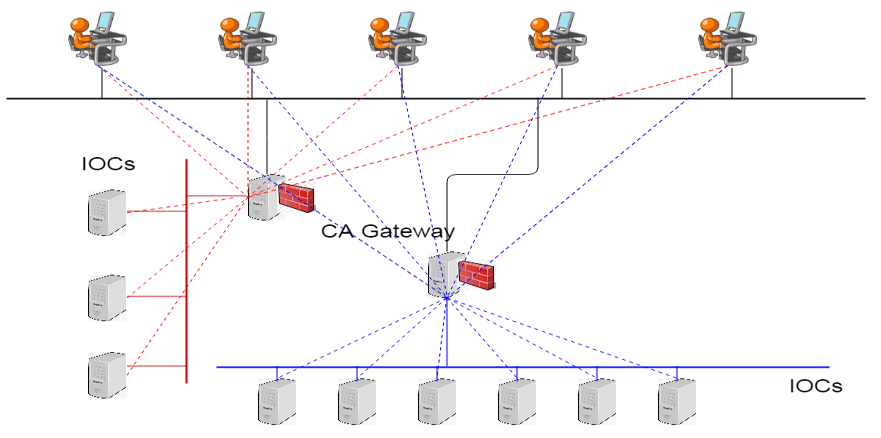
\includegraphics[width=1\textwidth]{./images/gateway.png}
	\caption{
		Gateway 구성
	}
	\label{fig:gateway}   
\end{figure}
\hfil\break

\chapter{EPICS v4 PVAccess Gateway Prototype 구현}
\section{EPICS Version 4 PVAccess}
EPICS 버전 4는 대형 실험 시설의 제어 시스템 및 온라인 과학 서비스를 작성하기위한 소프트웨어 툴킷입니다.EPICS Version 4는 현재 EPICS 버전 중 성능에 있어서 가장 우수하며, 다양한 기능을 갖는다. 또한, EPICS Version 4는 기존 EPICS Version 3에 추가적으로 복잡한 Scientfic complex 데이터 구조를 사용자 정의가 가능하도록 구현되는 Service 관점의 아키텍쳐로 확장된다. 더욱 넓은 의미로, EPICS는 공동으로 개발되고 전 세계에서 분산 소프트 실시간 제어 시스템을 작성하는 데 사용되는 일련의 오픈 소스 소프트웨어 도구, 라이브러리 및 응용 프로그램이기도 하다.EPICS Version 4 는 관리 분산 데이터 수집, 서비스 지향 아키텍처 및 복잡한 데이터 구조를 지원합니다. EPICS V4 워킹 그룹은 EPICS V4 기반 프로토콜 및 소프트웨어의 표준에 대한 참조 구현, 정의 및 제공하기 위한  노력을 기울인다.

EPICS Version 4 is a set of software modules that add to the base of the EPICS toolkit for advanced control systems. Version 4 adds the possibility of process variable (PV) values of structured data, an introspection interface for dynamic typing plus some standard types, high-performance streaming, and a new front-end processing database for managing complex data I/O. A synchronous RPC-style facility has also been added so that the EPICS environment supports service-oriented architecture.

The new "pvDatabase" module of EPICS Version 4 implements a framework for a memory resident database of records defined in terms of pvData structures. Like the IOC database of classic EPICS, the records of pvDatabase can process on I/O events; unlike the IOC the records may be of any structure the engineer wishes, and may pull in data from any pvAccess-ible data source, plus Channel Access. pvDatabase images may be standalone, or hosted within an IOC, where they might interface directly to base records, asynchronous device driver support (asynDriver), or detector control (areaDetector). pvDatabase is then useful for complex optimal control tasks, data assembly, and preprocessing. Combined with pvAccess streaming, it can be used as the basis of a data processing pipeline.

In an EPICS installation it is expected that control and module support would be done with EPICS Base IOCs, possibly including the new version 4 modules for accessing the base IOC database (pvaSrv), and for processing complex data (pvDatabase). Middle layer and SOA operations would be done with standalone pvDatabase instances at host level, and with the RPC facility. Version includes support for protocol interoperability with Base IOCs.

EPICS Version 4 is composed of a number of core standards and APIs, reference implementations of those standards in C++ and Java, plus associated other components and tools. The intention is for the standards and APIs to go through a public review process, leading to published protocols and APIs that may be independently implemented.

The Developer Guide provides a description of the various modules that are provide with each EPICS V4 release.


Release 4.6
The latest release, v4.6 consists of the following modules:

pvDataJava and pvDataCPP
Minor changes since previous release
normativeTypesJava and normativeTypesCPP
Minor changes since previous release
pvAccessJava and pvAccessCPP
Minor changes since previous release
pvaClientJava and pvaClientCPP
More robust than previous release.
easyPva Java no longer supported.
pvDatabaseJava and pvDatabaseCPP
pvaSrv
Minor changes since last release.
pvaPy
Several changes since last release.
exampleJava and exampleCPP
Many new examples since last release

Several examples that were in pvaClient and pvDatabase have been moved to here.
A lot of changes were made to Developer Guide. It is a good way to understand the various v4.6 modules.



\section{동기 및 특성}
EPICS v3의 CA(channel access) gateway 구성요소와 유사하게 EPICS v4 PV(PVAccess) gateway 구성요소는 CA(v3)와 PV(v4)로 명명된 클라이언트 및 서버를 포함한 어플리케이션을 말한다.그것의 주된 기능은 IP 네트워크 경계를 가로지르는 proxy connection 이다. 이는 gateway의 클라이언트 측에서 서버(IOC) 를 보호하기 위하여 채널 이름을 고유하게 해석하고, 데이터의 update를 클라이언트로 보내는 작업을 gateway측으로 옮기는 역할을 한다. 이를 위하여 PV gateway는 더많은 네트워크 연결 및 컴퓨터 자원 할당이 가능한 장치가 사용되어야 한다. 

In a distributed control system, there are hundreds of nodes that are part of the
plant. These nodes make up the controllers and the operator consoles. There
are many clients that may want to view the state of equipment outside of the
control network. A “gateway” allows clients outside of the control system to
view the equipment while limiting the additional traffic on the control network.
The gateway marshals all external requests and makes only one request into the
control system. This limits the effect of external requests on the control system,
thus maintaining the determinism required for robust operation of a facility.

\section{Fuctional Requirements}
\subsection{Requirements Identification}
The component identifier of the PV Gateway is 'PVGW'. The requirement identifiers are formatted as \newline
\hfil\break

PVGW-REQ-\{req-category\}-\{req-number\} \newline

The requirement categories used in this document are:

\begin{center}
	\begin{longtable}[t]{>{\raggedleft\arraybackslash} p{3cm} |p{2cm}}
		\caption{Requirement Category}
		\label{table:req_cat}\\
		\toprule
		\texttt{Category} & \textbf{ID} \\
		\midrule
		\endfirsthead
		\toprule
		\texttt{Category} & \textbf{ID} \\
		\midrule
		\endhead
		\midrule \multicolumn{2}{r}{\tablename\ \thetable\ -- \textit{Continued on next page}} \\
		\bottomrule
		\endfoot
		\bottomrule
		\endlastfoot
		\texttt{Functional}  & F \\
		\texttt{External}  & I \\
		\texttt{Other}    & O \\
	\end{longtable}
\end{center}

\subsection{EPICS Network Protocol Requirements}
\subsubsection{PVGW-REQ-F-001 pvAccess Client}
The Gateway should be able to connect to internal servers using the pvAccess network protocol of EPICS V4.

\subsubsection{PVGW-REQ-F-002 pvAccess Server}
The Gateway should provide channels on the external network by means of the pvAccess network protocol of EPICS V4.

\subsubsection{PVGW-REQ-F-003 Configurable pvAccess Server}
It should be possible to configure if the pvAccess server (PVGW-REQ-F-002) is started. This configuration should be defined at start-up, and is not required to be changeable at runtime.

\subsubsection{PVGW-REQ-F-004 Redundant pvAccess Server Operation}
It should be possible to run multiple Gateways with identical configuration in parallel, to allow failover and load balancing. This mode should not require special configuration on the external clients.

\subsubsection{PVGW-REQ-F-011 Channel Access Client}
The Gateway should be able to connect to internal servers using the Channel Access network protocol of EPICS V3.

\subsubsection{PVGW-REQ-F-012 Channel Access Server}
The Gateway should provide channels on the external network by means of the Channel Access network protocol of EPICS V3.

\subsubsection{PVGW-REQ-F-013 Configurable Channel Access Server}
It should be possible to configure if the Channel Access server (PVGW-REQ-F-012) is started. This configuration should be defined at start-up, and is not required to be changeable at runtime.

\subsubsection{PVGW-REQ-F-021 Configurable Server Side Network Binding}
On machines with multiple network interfaces, the Gateway should allow configuration of the network interfaces that its server(s) bind to. This configuration should be defined at start-up, and is not required to be changeable at runtime.


\subsection{Data Flow Engine Requirements}

\subsubsection{PVGW-REQ-F-101 Full pvData Support}
The Gateway should support transport of all pvData structures without restrictions. No legal pvData type should require recompilation or restart of the Gateway.

\subsubsection{PVGW-REQ-F-102 Full Normative Type Support}
The Gateway should support transport of all Normative Type (NT) structures without restrictions. it must not depend on specific properties of any NT.

\subsubsection{PVGW-REQ-F-111 Low Latency for Large Structures/Arrays}
The Gateway should add minimal latency when forwarding large structures or arrays. Sending data to the external clients should start immediately, and not require data structures to be received completely.

\subsubsection{PVGW-REQ-F-112 Quality-of-Service Mechanisms}
The Gateway should implement mechanisms to avoid negative effects of connections with large structures and arrays on connections to other PVs on the same internal server.

\subsubsection{PVGW-REQ-F-121 Combine Sub-Structure Subscriptions}
The Gateway should be able to combine external clients' subscriptions to different sub-structures of the same channel into one subscription to the internal server.

\subsubsection{PVGW-REQ-F-122 Combine Request Configurations for Identical Subscriptions}
The Gateway should be able to combine external clients' request configurations (pvRequest) for subscriptions to identical sub-structures of the same channel into one subscription to the internal server.

\subsubsection{PVGW-REQ-F-131 Data Cache}
The Gateway should be able to cache data, so that data for replies to get operations and initial updates on new subscriptions from external clients may be taken from the cache.

\subsubsection{PVGW-REQ-F-132 Configurable Data Cache}
Application of the "Data Cache" feature (PVGW-REQ-F-131) to get operations should be configurable, both globally and specifically on a channel name/regex base.

\subsubsection{PVGW-REQ-F-141 Transparent Data Behavior}
The Gateway should act completely transparent. When comparing a direct connection to a PV with a connection through the Gateway, order and contents of received data should be the same.
This does not apply to get operations, when data caching (PVGW-REQ-131) is enabled. In that case, the values returned from the cache may be different from the values in the internal server

\subsubsection{PVGW-REQ-F-142 Transparent Out-of-Band Behavior}
The Gateway should act transparent with respect to out-of-band behavior. When comparing a direct connection to a PV with a connection through the Gateway, out-of-band situations (e.g., connection loss, reconnection, non-existent PV) should produce the same exceptions in the same order.

\subsubsection{PVGW-REQ-F-143 Transparent Timeout Behavior}
The Gateway should act transparent with respect to timeouts. When comparing a direct connection to a PV with a connection through the Gateway, timeouts defined by the external client should be honored in the same way.

\subsubsection{PVGW-REQ-F-151 Name Server}
If the Gateway receives a name resolution request from an external client for a channel that it already serves, it should send an immediate positive reply to the request without querying the internal servers. If the Gateway receives a name resolution request from an external client for a channel that it should serve, but lost connection to, it should send an immediate negative reply to the request without querying the internal servers. If the Gateway receives a name resolution request from an external client for a channel that it was not able find recently (within a configurable interval), it should send an immediate negative reply to the request without querying the internal servers.

\subsubsection{PVGW-REQ-F-161 Connection Cache}
The Gateway should cache connections, i.e. keep the channel connection open with subscription disabled, for a configurable time after the last external client disconnected.


\subsection{Authentication/Authorization Requirements}

\subsubsection{PVGW-REQ-F-201 Local AuthN/AuthZ}
The Gateway should support a local layer of authentication and authorization, where authN/authZ for requests is decided possibly using an independent authN/authZ server, but without querying the internal server.

\subsubsection{PVGW-REQ-F-202 Run-Time Configurable Local AuthN/AuthZ}
The "Local AuthN/AuthZ" feature (PVGW-REQ-F-201) should be configurable at run-time. Activating a new configuration should not require a restart of the Gateway. Connections whose authZ does not change by the new configuration should not be affected.

\subsubsection{PVGW-REQ-F-203 Proxy AuthN/AuthZ}
The Gateway should support proxy authentication and authorization, where authorization for requests is decided by querying the internal server, using the credentials supplied by the external client.

\subsubsection{PVGW-REQ-F-211 Transparent AuthZ Forwarding}
The Gateway should transparently forward authorization changes on the internal connections to its external clients.

\subsection{External Interface Requirements}
\subsubsection{PVGW-REQ-I-001 Statistics Data}
The Gateway should provide statistical and performance data as pvData NT structures.

\subsubsection{PVGW-REQ-I-002 Network Binding for Statistics Data}
On machines with multiple network interfaces, the Gateway should allow configuration of the network interfaces that the statistics data (PVGW-REQ-I-001) server(s) bind to, independent from the equivalent setting of the data server(s) (PVGW-REQ-F-021). This configuration should be defined at start-up, and is not required to be changeable at runtime.

\subsubsection{PVGW-REQ-I-011 Debugging Shell}
The Gateway should provide a shell for debugging purposes, allowing to inspect its internal structures and lists, trace requests, set up debug log output filtered by channel or external client or internal server, etc.

\subsection{Other Requirements}
\subsubsection{PVGW-REQ-O-001 Build Environment}
The Gateway component should compile in a standard EPICS V4 build environment, using the standard EPICS V4 tools and compilers.

\subsubsection{PVGW-REQ-O-002 Supported Platforms}
The Gateway should be supported on all host type architectures/platforms officially supported by EPICS V4.

\subsubsection{PVGW-REQ-O-003 SMP Support}
The Gateway should be able to make use of SMP architectures, distributing load onto the available CPUs.





\section{PVAccess Gateway 프로토타입 설계 및 구현}
\subsection{용어}

\subsubsection{IP}
Internet Protocol (v4 and/or v6)

\subsubsection{PV}
Process Variable. Addressable unit in PVA.

\subsubsection{PVA}
PVAccess network protocol

\subsubsection{GW}
Gateway

\subsubsection{CLI}
An arbitrary PVAccess client (end user or another gateway)

\subsubsection{GWS}
Gateway server side (CLI communicates with this)

\subsubsection{GWC}
Gateway client side (SRV communicates with this)

\subsubsection{SRV}
An arbitrary PVAccess server (may be another gateway)



\subsection{시험 결과}



















\clearpage

\bibliographystyle{unsrtnat}


\end{document}

